\chapter{Jogos similares}
\begin{figure}[h]
    \centering
    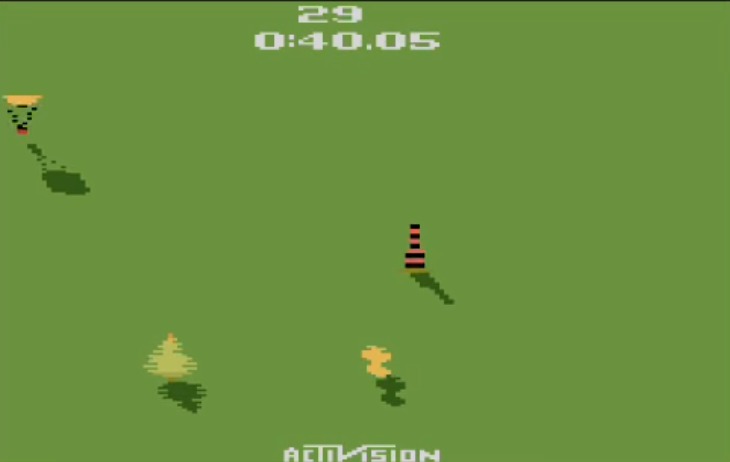
\includegraphics[width=0.7\textwidth]{sky-jinx.png}
    \caption{Sky Jinks (Atari 2600)\cite{jinks}}
\end{figure}
O Sky Jinks é semelhante ao BaffAttack pelo tema de aviação e pela mecânica de desvio de obstáculos. No Sky Jinks, o jogador pilota um avião em um percurso (na imagem à esquerda, o avião é o objeto laranja na parte inferior central), desviando de balões e outros obstáculos para chegar ao final no menor tempo possível. A necessidade de reflexos rápidos e controle constante da aeronave, assim como a visão top-down, são elementos que Sky Jinx compartilham com BaffAttack.

\begin{figure}[h]
    \centering
    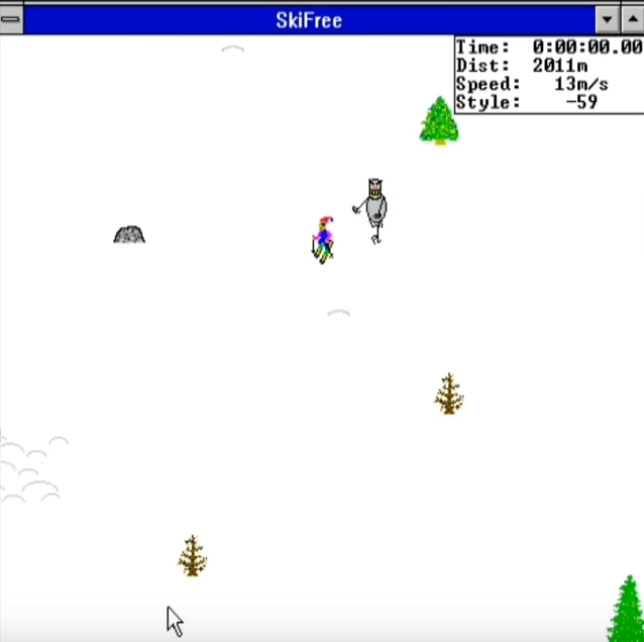
\includegraphics[width=0.6\textwidth]{ski-free.png}
    \caption{Ski Free (Windows 3.1)\cite{ski}}
\end{figure}
Pode parecer um jogo diferente à primeira vista, já que não é na temática de aviões, mas compartilha a mecânica de desvio de obstáculos e percurso pré-estabelecido. No "Ski Free", o jogador controla um esquiador que deve descer uma montanha enquanto evita obstáculos como árvores e outros esquiadores. Igual ao meu jogo, a posição do mouse para esquerda ou direita move o personagem.

\begin{figure}[h]
    \centering
    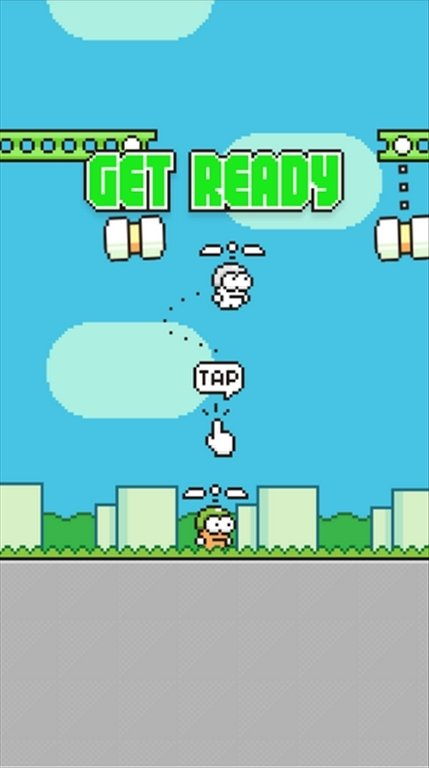
\includegraphics[width=0.4\textwidth]{swing-copters.jpg}
    \caption{Swing Copters (iOS e Android)}
\end{figure}
Swing Copters é um jogo bem mais atual que, assim como este jogo, exige precisão e reflexos rápidos. No Swing Copters, o jogador controla um personagem que voa com um helicóptero, desviando de obstáculos que surgem de forma imprevisível. A mecânica de controle do helicóptero, que lembra o controle de um avião, e a necessidade de desviar com precisão de obstáculos em um ambiente de jogo rápido e desafiante. Igual ao outro projeto do mesmo desenvolvedor, Flappy Bird, o jogo é extremamente simples visualmente, mas extremamente difícil. O BaffaAttack possui três níveis e considero que o nível fácil não muito complicado para terminar, mesmo para alguém que esteja jogando pela primeira vez.


